\chapter{Bağlantılılık}

Bağlantılılık, bir topolojik uzayın iki ayrı açık parçaya bölünememesi özelliğidir.
Yol-bağlantılılık daha güçlü bir kavramdır ve sürekli yolların varlığına dayanır.

%-------------------------------------------------------------------
\section{Konu}

\subsection{Sezgisel Giriş — ``Tek Parça mı, Kopuk mu?''}

Bağlantılılığı tek cümlede özetlemek gerekirse: \emph{bir uzayın iki ayrı açık
parçaya kesilememesidir.} Bir kâğıt parçasını düşünün; onu hiçbir yeri yırtmadan
iki ayrı açık parçaya bölemiyorsanız o kâğıt bağlantılıdır. Baştan iki ayrı
kâğıdınız varsa uzay bağlantısızdır.

\begin{figure}[ht]
  \centering
  \begin{tikzpicture}[font=\small, etiket/.style={font=\scriptsize}]
  % --- Sol: baglantili uzay (tek parca) ---
  \node[etiket] at (1.6,2.55) {\textbf{Bağlantılı}};
  \draw[blue!70!black, very thick, fill=blue!12, rounded corners=14pt]
    (0.2,0.4) ellipse (1.5 and 1.0);
  \node at (1.6,0.4) {$X$};
  \node[etiket, align=center] at (1.6,-1.05)
    {Tek parça: boş olmayan,\\$X$'ten farklı clopen küme \emph{yok}};

  % --- Orta: ayirici ok ---
  \draw[-{Stealth[length=2.6mm]}, thick] (3.5,0.4) -- (4.6,0.4)
    node[midway, above, etiket] {kopar};

  % --- Sag: baglantisiz uzay (iki ayri acik parca) ---
  \node[etiket] at (7.4,2.55) {\textbf{Bağlantısız}};
  \draw[teal!70!black, very thick, fill=teal!12, rounded corners=10pt]
    (5.6,0.4) ellipse (0.95 and 0.85);
  \node at (6.05,0.4) {$U$};
  \draw[orange!80!black, very thick, fill=orange!14, rounded corners=10pt]
    (8.4,0.4) ellipse (0.95 and 0.85);
  \node at (8.75,0.4) {$V$};
  \node[etiket, align=center] at (7.4,-1.05)
    {$X = U \sqcup V$,\quad $U,V$ açık ve boş değil\\
     ikisi de clopen $\Rightarrow$ bağlantısız};
\end{tikzpicture}

  \caption{Bağlantılı (tek parça) ile bağlantısız ($X = U \sqcup V$, iki ayrı
    clopen parça) arasındaki fark.}
\end{figure}

Bu ``kesilememe'' fikrinin teknik karşılığı \textbf{clopen ayrılma}dır: uzay
bağlantısızdır ancak ve ancak boş olmayan, uzayın tamamından farklı, hem açık hem
kapalı (\emph{clopen}) bir küme varsa.

\begin{sezgi}
``Bağlantılı'' uzayın tek parça olmasıdır; ``yol-bağlantılı'' ise herhangi iki
noktayı sürekli bir yol ile birleştirebilmektir. İkinci kavram birincisinden
\emph{daha güçlü}: yol kurabiliyorsanız zaten tek parçasınızdır, ama tek parça
olmak her zaman yol kurabildiğiniz anlamına gelmez (topolojist sinüs eğrisi).
\end{sezgi}

\subsection{Bağlantılılık Kavramları}

\begin{definition}[Bağlantılı Uzay]
$(X, \tau)$ uzayı \textbf{bağlantılı} ise: $X = U \cup V$, $U \cap V = \emptyset$,
$U,V$ açık $\Rightarrow U = \emptyset$ veya $V = \emptyset$.
\end{definition}

\begin{definition}[Yol-Bağlantılı]
$\forall x,y \in X$: $\exists$ sürekli $f:[0,1] \to X$, $f(0) = x$, $f(1) = y$.
\end{definition}

\begin{table}[h]
\centering
\begin{tabular}{ll}
\toprule
\textbf{Kavram} & \textbf{Özellik} \\
\midrule
Bağlantılı & Clopen bölme yok \\
Yol-bağlantılı & Her iki nokta arasında sürekli yol var \\
Ark-bağlantılı & Yol-bağlantılı; yollar enjektif \\
Lokal bağlantılı & Her noktanın bağlantılı komşuluğu \\
Tamamen bağlantısız & Her bağlantılı alt küme tek noktadır \\
\bottomrule
\end{tabular}
\caption{Bağlantılılık hiyerarşisi}
\end{table}

\textbf{Sıralama:} Ark-bağlantılı $\Rightarrow$ Yol-bağlantılı $\Rightarrow$ Bağlantılı.

\subsection{Clopen Ayrılma}

$X$ bağlantısız $\Leftrightarrow$ boş olmayan trivial olmayan bir clopen $A \subsetneq X$ vardır.

\subsection{Bağlantılı Bileşenler}

Bir uzayı, içerme bakımından \textbf{en büyük} bağlantılı alt kümelerine
ayırabiliriz; bunlara \emph{bağlantılı bileşenler} denir. Bileşenler $X$'i örten,
ayrık parçalardır. Uzay bağlantılıdır $\Leftrightarrow$ tek bir bileşeni vardır.

\begin{figure}[ht]
  \centering
  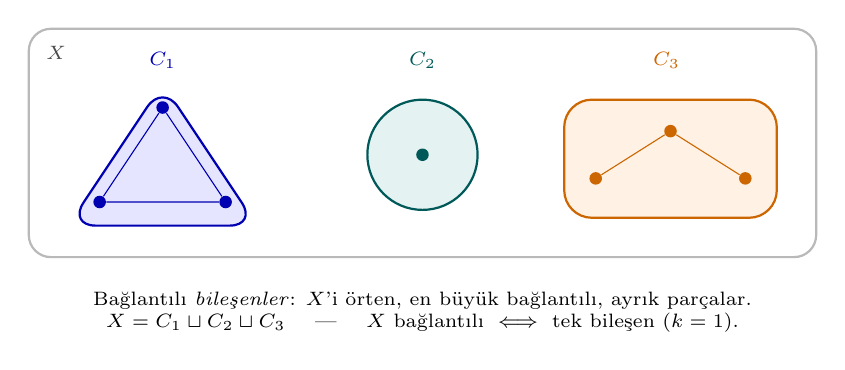
\begin{tikzpicture}[font=\small, etiket/.style={font=\scriptsize},
    nokta/.style={circle, fill, inner sep=1.6pt}]
  % ust cerceve: bir uzayin 3 ayri "ada"si = 3 baglantili bilesen
  \draw[gray!55, thick, rounded corners=8pt] (-0.5,-1.3) rectangle (9.5,1.6);
  \node[gray!60!black, etiket, anchor=north west] at (-0.4,1.5) {$X$};

  % Bilesen 1: ucgen (baglantili)
  \node[blue!70!black, etiket] at (1.2,1.2) {$C_1$};
  \draw[blue!70!black, thick, fill=blue!10, rounded corners=10pt]
    (0.0,-0.9) -- (2.4,-0.9) -- (1.2,0.9) -- cycle;
  \node[nokta, blue!70!black] (a1) at (0.4,-0.6) {};
  \node[nokta, blue!70!black] (a2) at (2.0,-0.6) {};
  \node[nokta, blue!70!black] (a3) at (1.2,0.6) {};
  \draw[blue!70!black] (a1)--(a2)--(a3)--(a1);

  % Bilesen 2: tek nokta (izole)
  \node[teal!70!black, etiket] at (4.5,1.2) {$C_2$};
  \draw[teal!70!black, thick, fill=teal!10] (4.5,0.0) circle (0.7);
  \node[nokta, teal!70!black] at (4.5,0.0) {};

  % Bilesen 3: yol (baglantili)
  \node[orange!80!black, etiket] at (7.6,1.2) {$C_3$};
  \draw[orange!80!black, thick, fill=orange!10, rounded corners=10pt]
    (6.3,-0.8) rectangle (9.0,0.7);
  \node[nokta, orange!80!black] (b1) at (6.7,-0.3) {};
  \node[nokta, orange!80!black] (b2) at (7.65,0.3) {};
  \node[nokta, orange!80!black] (b3) at (8.6,-0.3) {};
  \draw[orange!80!black] (b1)--(b2)--(b3);

  \node[etiket, align=center] at (4.5,-2.0)
    {Bağlantılı \emph{bileşenler}: $X$'i örten, en büyük bağlantılı, ayrık parçalar.\\
     $X = C_1 \sqcup C_2 \sqcup C_3$ \quad — \quad $X$ bağlantılı $\iff$ tek bileşen ($k=1$).};
\end{tikzpicture}

  \caption{Bağlantılı bileşenler: $X = C_1 \sqcup C_2 \sqcup C_3$; her parça en
    büyük bağlantılı alt kümedir. $X$ bağlantılı $\iff$ tek bileşen.}
\end{figure}

\begin{karsiornek}
\textbf{Topolojist sinüs eğrisi — bağlantılı ama yol-bağlantılı değil.}
$S = \{(x, \sin\tfrac{1}{x}) : 0 < x \le 1\} \cup (\{0\}\times[-1,1])$ kümesini
ele alın. Sağdaki eğri $x \to 0^+$ giderken sonsuz hızla salınır ve soldaki dikey
segmente keyfi yakın olur; bu yüzden $S$ \textbf{bağlantılıdır}. Ama dikey
segmentteki bir noktayı eğri üzerindeki bir noktaya bağlayan \emph{sürekli} bir
yol \textbf{yoktur} --- yol $x=0$'a yaklaşırken sinüs salınımı yakınsamayı
engeller. Demek ki $S$ bağlantılı, fakat yol-bağlantılı değildir.
\end{karsiornek}

\begin{figure}[ht]
  \centering
  \begin{tikzpicture}[font=\small, etiket/.style={font=\scriptsize}]
  % topolojist sinus egrisi: y = sin(1/x), x in (0, ~0.9], + dikey segment {0}x[-1,1]
  % dikey limit segmenti
  \draw[blue!70!black, very thick] (0,-1) -- (0,1);
  \node[blue!60!black, etiket, left=2pt] at (0,0) {$\{0\}\times[-1,1]$};

  % sin(1/x) egrisi: gercek x in (0, 0.9], yatay olcek 3.3 -> grafik x ekseni
  % yakin x=0 icin yogun ornekleme (sonsuz salinim gorunur olsun)
  \draw[orange!80!black, very thick, domain=0.028:0.9, samples=900, smooth, variable=\x]
    plot ({\x*3.3},{sin((1/\x) r)});
  \node[orange!75!black, etiket] at (2.05,1.45) {$y=\sin\!\left(\tfrac{1}{x}\right),\; x>0$};

  % salinim oku
  \draw[-{Stealth[length=2.4mm]}, red!70!black, thick] (0.95,-1.35) -- (0.2,-1.35);
  \node[red!70!black, etiket, align=center] at (1.7,-1.45)
    {$x\to 0^+$ iken sonsuz salınım};

  \node[etiket, align=center, fill=blue!5, rounded corners, inner sep=4pt]
    at (1.5,-2.35)
    {\textbf{Bağlantılı} ama \textbf{yol-bağlantılı değil:} sağdaki eğri ile soldaki
     dikey segmenti\\ birleştiren \emph{sürekli} bir yol yoktur (salınım yakınsamayı engeller).};
\end{tikzpicture}

  \caption{Topolojist sinüs eğrisi: $x\to 0^+$ iken sonsuz salınım. Eğri ile
    dikey limit segmenti arasında sürekli yol kurulamaz.}
\end{figure}

%-------------------------------------------------------------------
\section{Teoremler}

\begin{theorem}
Bağlantılı küme süreklilik altında bağlantılıdır:
$f: X \to Y$ sürekli, $X$ bağlantılı $\Rightarrow f(X)$ bağlantılı.
\end{theorem}

\begin{proof}[İspat eskizi]
$f(X)$ bağlantısız olsaydı, $f(X) = U \sqcup V$ biçiminde boş olmayan, ayrık, açık
iki kümeye ayrılırdı. Süreklilikten $f^{-1}(U)$ ve $f^{-1}(V)$ açıktır; ayrıktır;
birleşimleri $X$'tir ve ikisi de boş değildir. Bu, $X$'in bir clopen ayrılmasıdır
--- $X$'in bağlantılılığıyla çelişir. Demek ki $f(X)$ bağlantılıdır.
\end{proof}

\begin{theorem}
Yol-bağlantılı $\Rightarrow$ bağlantılı. Tersi genel olarak yanlış.
(Karşı örnek: Topolojist sinüs eğrisi.)
\end{theorem}

\begin{proof}[İspat eskizi]
$X$ yol-bağlantılı ama bağlantısız olsaydı, $X = U \sqcup V$ clopen ayrılması
olurdu. $x \in U$, $y \in V$ alıp $f:[0,1]\to X$, $f(0)=x$, $f(1)=y$ sürekli
yolunu kuralım. $[0,1]$ bağlantılı olduğundan görüntü $f([0,1])$ de bağlantılıdır;
ama bu görüntü $U$ ve $V$ tarafından gerçek bir clopen ayrılmaya uğrar --- çelişki.
Ters yön yanlıştır: topolojist sinüs eğrisi bağlantılı, ama yol-bağlantılı değildir.
\end{proof}

\begin{theorem}[Ara Değer Teoremi]
$f: X \to \mathbb{R}$ sürekli, $X$ bağlantılı $\Rightarrow f(X)$ bir aralıktır.
\end{theorem}

\begin{proof}[İspat eskizi]
$f(X) \subseteq \mathbb{R}$ bağlantılıdır (önceki teorem). $\mathbb{R}$'de
bağlantılı kümeler tam olarak aralıklardır; demek ki $f(X)$ bir aralıktır.
$a, b \in f(X)$ ise aralık özelliğinden $[a,b] \subseteq f(X)$; yani her
$c \in [a,b]$ için $f^{-1}(c) \neq \emptyset$.
\end{proof}

\begin{theorem}
Gerçek doğru $\mathbb{R}$'de bağlantılı alt kümeler tam olarak aralıklardır.
\end{theorem}

\begin{proof}[İspat eskizi]
(Aralık $\Rightarrow$ bağlantılı) Bir $I$ aralığı $U \sqcup V$ clopen ayrılmasına
uğrasaydı, $a\in U$, $b\in V$ ($a<b$) alıp $c=\sup\{x\in U : x\le b\}$ tanımlanır;
$c$'nin hangi parçada olduğu hem açıklık hem kapalılıkla çelişir. (Bağlantılı
$\Rightarrow$ aralık) $S$ aralık değilse $a<c<b$, $a,b\in S$, $c\notin S$ olan bir
$c$ vardır; o zaman $(-\infty,c)\cap S$ ve $(c,\infty)\cap S$ bir clopen ayrılma verir.
\end{proof}

%-------------------------------------------------------------------
\section{Algoritmalar}

\subsection{Sonlu Bağlantılılık — $O(|\tau|^2)$}

\begin{algorithm}
\caption{BagliMi$(X, \tau)$}
\begin{algorithmic}[1]
\For{each non-empty $A \subsetneq X$}
    \If{$A \in \tau$ \textbf{and} $X \setminus A \in \tau$}
        \State \Return False \Comment{Clopen bölme bulundu}
    \EndIf
\EndFor
\State \Return True
\end{algorithmic}
\end{algorithm}

Karmaşıklık: $O(|\tau|^2)$ — clopen küme taraması.

%-------------------------------------------------------------------
\section{pytop API}

\begin{lstlisting}[language=Python]
from pytop import (
    is_connected,
    is_path_connected,
    is_locally_connected,
    is_totally_disconnected,
)
\end{lstlisting}

%-------------------------------------------------------------------
\section{Örnekler}

\subsection*{Örnek 5.1 — Sierpiński: Bağlantılı}

\begin{lstlisting}[language=Python]
s = sierpinski_space()
print("connected?", is_connected(s).status)
print("path_connected?", is_path_connected(s).status)
\end{lstlisting}

\begin{verbatim}
connected?       true
path_connected?  unknown
\end{verbatim}

\subsection*{Örnek 5.2 — Ayrık Topoloji: Tamamen Bağlantısız}

\begin{lstlisting}[language=Python]
d = discrete_topology(1, 2, 3)
print("connected?", is_connected(d).status)
print("totally_disconn?", is_totally_disconnected(d).status)
\end{lstlisting}

\begin{verbatim}
connected?          false
totally_disconn?    true
\end{verbatim}

\subsection*{Örnek 5.3 — Gerçek Doğru ve [0,1]}

\begin{lstlisting}[language=Python]
rl = real_line_metric()
ui = closed_unit_interval_metric()
print("R connected?", is_connected(rl).status)
print("[0,1] path_connected?", is_path_connected(ui).status)
\end{lstlisting}

\begin{verbatim}
R connected?          true
[0,1] path_connected? true
\end{verbatim}

\subsection*{Örnek 5.4 — Ark / Yol / Bağlantı Hiyerarşisi}

Hiyerarşi \textbf{Ark $\Rightarrow$ Yol $\Rightarrow$ Bağlantılı} idi. pytop bu üç
düzeyi ayrı ayrı sorgular; bazı uzaylarda bir düzey \texttt{true}, diğeri
\texttt{unknown} döner --- pytop yalnızca \emph{kanıtlayabildiğini} bildirir.

\begin{lstlisting}[language=Python]
from pytop import (indiscrete_topology, real_line_metric, discrete_topology,
                   is_arc_connected, is_path_connected, is_connected)

for name, sp in [("Indiscrete(2)", indiscrete_topology(1, 2)),
                 ("R", real_line_metric()),
                 ("Discrete(3)", discrete_topology(1, 2, 3))]:
    print(f"{name:14s} connected={is_connected(sp).status:6s} "
          f"path={is_path_connected(sp).status:8s} arc={is_arc_connected(sp).status}")
\end{lstlisting}

\begin{verbatim}
Indiscrete(2)  connected=true   path=unknown  arc=true
R              connected=true   path=true     arc=unknown
Discrete(3)    connected=false  path=unknown  arc=false
\end{verbatim}

\subsection*{Örnek 5.5 — Tek Çağrıyla Çoklu Sorgu: \texttt{analyze\_connectedness}}

\texttt{analyze\_connectedness(space, property\_name)} tek bir dağıtıcı sunar;
geçerli adlar: \texttt{connected}, \texttt{path\_connected},
\texttt{locally\_connected}, \texttt{totally\_disconnected}, \texttt{arc\_connected}.

\begin{lstlisting}[language=Python]
from pytop import analyze_connectedness, sierpinski_space

s = sierpinski_space()
for prop in ["connected", "path_connected", "locally_connected",
             "totally_disconnected", "arc_connected"]:
    print(f"  {prop:22s}: {analyze_connectedness(s, prop).status}")
\end{lstlisting}

\begin{verbatim}
  connected             : true
  path_connected        : unknown
  locally_connected     : unknown
  totally_disconnected  : false
  arc_connected         : false
\end{verbatim}

Sierpiński bağlantılıdır ve tamamen bağlantısız \emph{değildir} --- tutarlı,
çünkü (tek noktadan büyük) bağlantılı bir uzay tamamen bağlantısız olamaz.

\subsection*{Örnek 5.6 — Clopen Ayrılmayı Elle Kurmak}

$X=\{1,2,3,4\}$ üzerinde $U=\{1,2\}$, $V=\{3,4\}$ taban alınırsa ikisi de clopen
olur; $X = U \sqcup V$ bir ayrılmadır. İç içe açıklar ise bölme vermez.

\begin{lstlisting}[language=Python]
from pytop import make_topology, is_connected, is_totally_disconnected

X = make_topology({1, 2, 3, 4}, {1, 2}, {3, 4})       # clopen bölme
print("split connected?", is_connected(X).status)
print("split totally_disconn?", is_totally_disconnected(X).status)

Y = make_topology({1, 2, 3}, {1}, {1, 2}, {1, 2, 3})  # ic ice, bölme yok
print("nested connected?", is_connected(Y).status)
\end{lstlisting}

\begin{verbatim}
split connected?        false
split totally_disconn?  false
nested connected?       true
\end{verbatim}

İlk uzay bağlantısız (clopen bölme var) ama \emph{tamamen} bağlantısız değil:
$\{1,2\}$ içinde clopen bölme yoktur. İkinci uzay iç içe açıklardan oluşur;
gerçek clopen bölme kurulamaz, bu yüzden bağlantılıdır.

%-------------------------------------------------------------------
\section{Alıştırmalar}

\subsection*{Kodlama}

\begin{enumerate}[label=K\arabic*.]
\item \texttt{make\_topology(\{1,2,3\},\{1\},\{2,3\})} için \texttt{is\_connected} hesaplayın.
\item \texttt{finite\_chain\_space(4)} zincirinin bağlantılı olup olmadığını kontrol edin.
\item İki noktalı ayrık ve indiscrete uzaylar üzerinde \texttt{is\_connected},
      \texttt{is\_path\_connected} karşılaştırın.
\item \texttt{indiscrete\_topology(1,2)} ve \texttt{real\_line\_metric()} için
      \texttt{is\_arc\_connected} ve \texttt{is\_path\_connected} çıktılarını
      karşılaştırın. Hangi uzayda hangi düzey \texttt{unknown} döner?
      \ipucu{Örnek 5.4.}
\item \texttt{discrete\_topology(1,2,3)} için
      \texttt{analyze\_connectedness(d, "connected")} ve
      \texttt{analyze\_connectedness(d, "totally\_disconnected")} çağırın; iki
      sonucun neden tutarlı olduğunu açıklayın. \ipucu{Örnek 5.5.}
\end{enumerate}

\subsection*{Teori}

\begin{enumerate}[label=T\arabic*.]
\item Bağlantılı + sürekli $\Rightarrow$ görüntü bağlantılı teoremini ispatlayın.
\item Yol-bağlantılı $\Rightarrow$ bağlantılı implicasyonunu ispatlayın.
\item Topolojist sinüs eğrisinin neden bağlantılı \emph{ama} yol-bağlantılı
      olmadığını açıklayın: dikey segmentten eğriye sürekli bir yol varsayıp
      çelişkiye ulaşın. \ipucu{\S1 karşı-örnek kutusu + sinüs eğrisi figürü.}
\end{enumerate}
